\documentclass[border=10pt]{standalone}
\usepackage[svgnames]{xcolor}
\usepackage{amsmath}
\usepackage{pgfplots}
\pgfplotsset{compat=newest}
\usepackage[sfdefault]{FiraSans}
\usepackage{FiraMono}
\renewcommand*\familydefault{\sfdefault}
\begin{document}
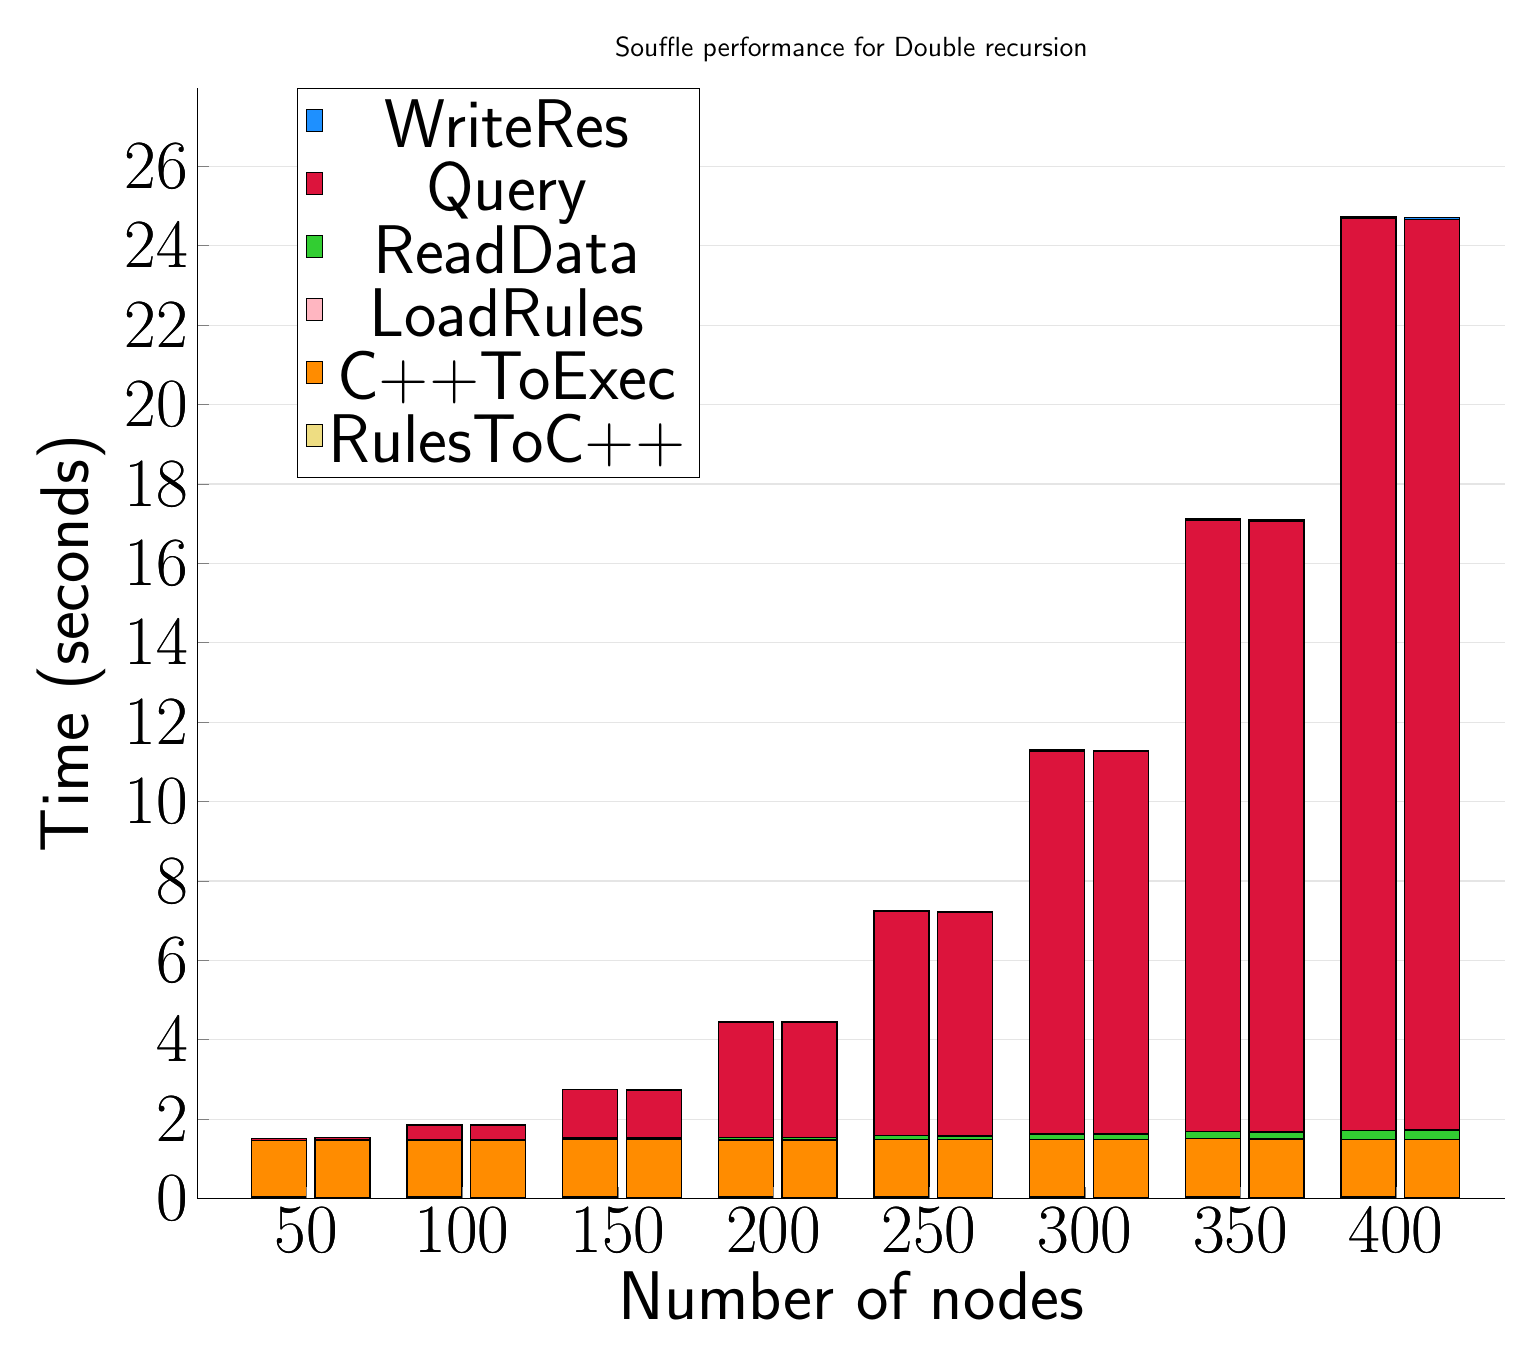
\begin{tikzpicture}
\begin{axis}[
   ybar stacked,
   title={Souffle performance for Double recursion},
   bar shift=-10pt,
   width=1.5\textwidth,
   bar width=0.7cm,
   ymajorgrids, tick align=inside,
   major grid style={draw=gray!20},
   xtick=data,
   ymin=0, ymax=27.977500000000003,
   axis x line*=bottom,
   axis y line*=left,
   enlarge x limits=0.1,
   legend style={
       at={(0.23, 1)},
       anchor=north,
       legend columns=1,
       font=\Huge,
   },
   ylabel={Time (seconds)},
   xlabel={Number of nodes},
   label style={font=\Huge},
   tick label style={font=\Huge},
]
\addlegendimage{fill=DodgerBlue, draw=black, line width=0.2pt}
\addlegendentry{WriteRes}
\addlegendimage{fill=Crimson, draw=black, line width=0.2pt}
\addlegendentry{Query}
\addlegendimage{fill=LimeGreen, draw=black, line width=0.2pt}
\addlegendentry{ReadData}
\addlegendimage{fill=LightPink, draw=black, line width=0.2pt}
\addlegendentry{LoadRules}
\addlegendimage{fill=DarkOrange, draw=black, line width=0.2pt}
\addlegendentry{C++ToExec}
\addlegendimage{fill=LightGoldenrod, draw=black, line width=0.2pt}
\addlegendentry{RulesToC++}
\addplot +[fill=LightGoldenrod, draw=black, line width=0.5pt] coordinates {
    (50, 0.03900003433227539)
    (100, 0.039999961853027344)
    (150, 0.04200000762939453)
    (200, 0.04100000858306885)
    (250, 0.04100000858306885)
    (300, 0.04200003147125244)
    (350, 0.041999983787536624)
    (400, 0.040999984741210936)
};
\addplot +[fill=DarkOrange, draw=black, line width=0.5pt] coordinates {
    (50, 1.4170000076293945)
    (100, 1.417999839782715)
    (150, 1.4490000247955321)
    (200, 1.430999994277954)
    (250, 1.4490000009536743)
    (300, 1.446999979019165)
    (350, 1.4710000038146973)
    (400, 1.4440000295639037)
};
\addplot +[fill=LightPink, draw=black, line width=0.5pt] coordinates {
    (50, 6.0920699999999994e-05)
    (100, 0.000101975)
    (150, 8.37042e-05)
    (200, 9.6121e-05)
    (250, 4.69584e-05)
    (300, 9.67417e-05)
    (350, 6.073749999999999e-05)
    (400, 0.00011145819999999998)
};
\addplot +[fill=LimeGreen, draw=black, line width=0.5pt] coordinates {
    (50, 0.005247118)
    (100, 0.0196616)
    (150, 0.03925768)
    (200, 0.06528643999999999)
    (250, 0.09532794)
    (300, 0.1358404)
    (350, 0.17973299999999998)
    (400, 0.23519050000000002)
};
\addplot +[fill=Crimson, draw=black, line width=0.5pt] coordinates {
    (50, 0.05645256)
    (100, 0.371263)
    (150, 1.214719)
    (200, 2.8969940000000003)
    (250, 5.644607000000001)
    (300, 9.646623000000002)
    (350, 15.398140000000001)
    (400, 22.977500000000003)
};
\addplot +[fill=DodgerBlue, draw=black, line width=0.5pt] coordinates {
    (50, 0.0008633789999999998)
    (100, 0.002878721)
    (150, 0.007174150999999999)
    (200, 0.01116645)
    (250, 0.01730473)
    (300, 0.02472958)
    (350, 0.034022699999999996)
    (400, 0.04580653)
};
\end{axis}
\begin{axis}[
   ybar stacked,
   bar shift=13pt,
   width=1.5\textwidth,
   bar width=0.7cm,
   ymajorgrids, tick align=inside,
   major grid style={draw=none},
   xtick=data,
   ymin=0, ymax=27.977500000000003,
   axis x line*=none,
   axis y line*=none,
   enlarge x limits=0.1,
   label style={font=\Huge},
   tick label style={font=\Huge},
]
\addplot +[fill=LightGoldenrod, draw=black, line width=0.5pt] coordinates {
    (50, 0.030000000000000006)
    (100, 0.030000000000000006)
    (150, 0.030000000000000006)
    (200, 0.030000000000000006)
    (250, 0.030000000000000006)
    (300, 0.030000000000000006)
    (350, 0.030000000000000006)
    (400, 0.030000000000000006)
};
\addplot +[fill=DarkOrange, draw=black, line width=0.5pt] coordinates {
    (50, 1.4389999999999998)
    (100, 1.4369999999999998)
    (150, 1.4579999999999997)
    (200, 1.4469999999999996)
    (250, 1.452)
    (300, 1.4579999999999997)
    (350, 1.4680000000000002)
    (400, 1.464)
};
\addplot +[fill=LightPink, draw=black, line width=0.5pt] coordinates {
    (50, 6.050000000000001e-05)
    (100, 0.000101)
    (150, 8.31e-05)
    (200, 9.540000000000001e-05)
    (250, 4.6500000000000005e-05)
    (300, 9.420000000000001e-05)
    (350, 6.03e-05)
    (400, 0.00011080000000000001)
};
\addplot +[fill=LimeGreen, draw=black, line width=0.5pt] coordinates {
    (50, 0.0052462)
    (100, 0.0196514)
    (150, 0.0390651)
    (200, 0.0642769)
    (250, 0.0943064)
    (300, 0.1339607)
    (350, 0.17817019999999997)
    (400, 0.23433569999999998)
};
\addplot +[fill=Crimson, draw=black, line width=0.5pt] coordinates {
    (50, 0.0564302)
    (100, 0.37112169999999994)
    (150, 1.211378)
    (200, 2.8933929999999997)
    (250, 5.637921)
    (300, 9.635805)
    (350, 15.38324)
    (400, 22.933910000000004)
};
\addplot +[fill=DodgerBlue, draw=black, line width=0.5pt] coordinates {
    (50, 0.000863)
    (100, 0.0028777000000000004)
    (150, 0.0064158999999999996)
    (200, 0.011057899999999999)
    (250, 0.017295399999999995)
    (300, 0.024711200000000006)
    (350, 0.033670900000000004)
    (400, 0.0450793)
};
\end{axis}
\end{tikzpicture}

\end{document}
